\documentclass[addpoints,12pt]{exam}
%\documentclass[12pt]{article}
\usepackage[letterpaper, margin=0.75in]{geometry}
\usepackage{graphicx}
\usepackage{enumitem}
\usepackage{booktabs}
\usepackage{tabularx}
\usepackage{color}
\usepackage{wrapfig}

\begin{document}
\footer{}{Page \thepage\ of \numpages}{}

\begin{flushright}
\makebox[0.5\textwidth]{\large Name:\enspace\hrulefill}
\vspace{0.1in}

\makebox[0.5\textwidth]{\large Name:\enspace\hrulefill}
\vspace{0.1in}

\makebox[0.5\textwidth]{\large Name:\enspace\hrulefill}
\vspace{0.1in}
\end{flushright}

\vspace{0.2in}

\begin{center}

\includegraphics[width=10cm]{../images/logo.png}
\end{center}

\begin{center}
\noindent{\LARGE Conceptual Physics \\ First Partial Test\\ \textbf{GROUP} \\ March 30, 2018 \\}
\end{center}

\vspace{0.5in}

\begin{large}
You are free to use all notes on your two-sided cheat sheet. There are extra blank sheets at the end, which can be used for calculations, and if you require more please ask and be sure to include them when you hand back the test. Please be sure to include all your work and calculations.

Some useful geometric quantities for this test may include:
\begin{eqnarray}
\textrm{Area of a Circle} &=& \pi\times(\textrm{radius})^2 \nonumber \\
\textrm{Area of a Triangle} &=& \frac{1}{2}\textrm{base}\times\textrm{height}  \nonumber \\
\textrm{Area of a Rectangle} &=& \texttt{base}\times\textrm{height}\nonumber
\end{eqnarray}

There are \numquestions ~ problems for a total of \numpoints ~ points. (One of the questions is a bonus though.)

You will have \textbf{1h 15 minutes} to complete the test (which translates to about 15 minutes per question).

\textbf{I will randomly pick 1 test per group, and the entire group will receive that grade: It is therefore vital that everyone in the group be involved.}

\end{large}
\vspace{0.2in}

 
\clearpage

\begin{flushright}
Score: \hspace{0.2in} / \numpoints ~ points
\end{flushright}

\begin{questions}
\question \textbf{Binary Star Systems:} In solar systems like ours, there is one star (our sun) orbited by planets. However, other systems exist in which there are \textit{two} stars orbiting each other: These are known as \textit{binary star systems.} In binary star systems, both stars follow a (roughly) elliptical path. In the diagram below, images (I), (II), (III) and (IV) show snapshots in time of 2 stars in a binary system as they orbit each other. Use these images to answer the following questions. \textbf{For each question, please also \textit{explain your answer}.}

\begin{center}\input{../images/binary_star.pdf_tex}\end{center}

\begin{parts}
\part[2] At which instant (I, II, III, IV) is the \textit{gravitational force} between the two stars the \textit{greatest}? \textbf{Why?}
	\vspace{1in}
\part[2] At which instant (I, II, III, IV) is the \textit{gravitational potential energy} between the two stars the \textit{greatest}? \textbf{Why?}
	\vspace{1in}
\part[2] Assume energy is conserved in a binary system. At which instant (if any) is the \textit{speed} of the two stars the \textit{greatest}? \textbf{Why?}
	\vspace{1in}
\end{parts}

\clearpage

\question \textbf{Rutherford Experiment:} Also called the Geiger-Marsden experiment, was a landmark experiment that proved atoms contained a nucleus where the positive charge (and most of the mass) is concentrated. This was accomplished by bombarding very thin gold foils with ``alpha particles" (2 protons and 2 neutrons stuck together) and observing how the particles were deflected. The figure below shows an incoming alpha particle (positive charge) approaching a gold nucleus (also positively charged) and being deflected by their mutual repulsion. The gold nucleus remains nearly stationary during the event. Different parts of the particle's trajectory are labelled, and please use them to answer the following questions. \textbf{For each question, please also \textit{explain your answer}.}
	
	\noindent\begin{center}\input{../images/rutherford.pdf_tex}\end{center}
	
	\begin{parts}
	\part[2] At what point(s) during its trajectory (I, II, III, IV, V) does the alpha particle feel an electrical force, due to its interaction with the gold nucleus? \textbf{Why?}
		\vspace{1in}
	\part[2] At what point(s) during its trajectory (I, II, III, IV, V) does the alpha particle experience the \textit{greatest electric force}? \textbf{Why?}
		\vspace{1in}
	\part[2] At what point(s) during its trajectory (if any) does the alpha particle have the \textit{greatest electric potential energy}?\textbf{ Why?}
		\vspace{1in}
	\end{parts}

\clearpage
\question \textbf{Nuclear Fission:} Uranium is a radioactive element used as an energy source in nuclear reactors. When a uranium nucleus is bombarded with a neutron, it splits apart forming 2 other atoms, and in the process releases lots of nuclear potential energy (and more neutrons to continue the process).

\begin{center}
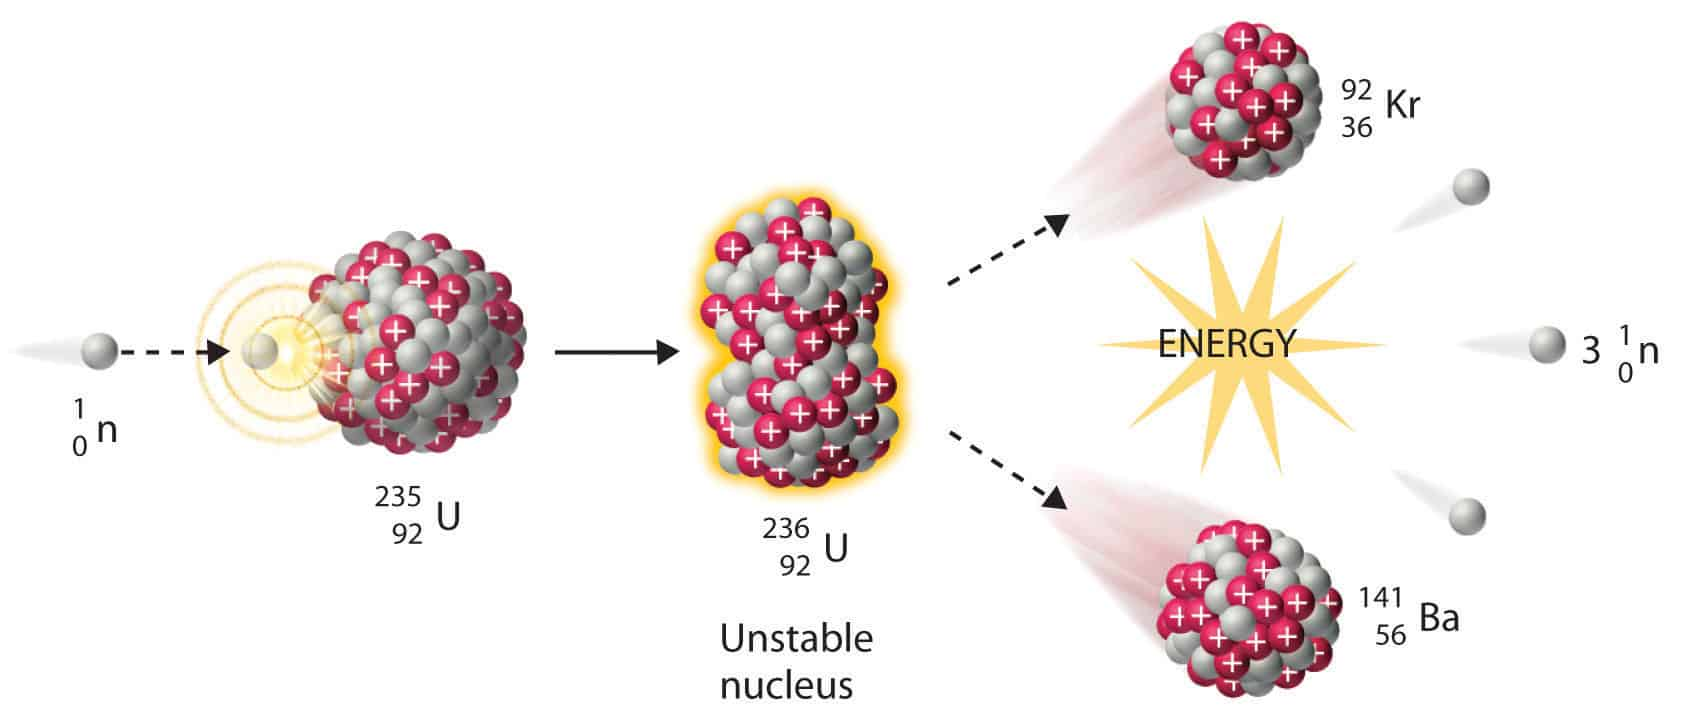
\includegraphics[width=0.8\textwidth]{../images/nuclear_fission.jpg}
\end{center}

\begin{parts}
	\part[2] The mass of 1 uranium atom is $4\times 10^{-22}$g. If a nuclear reactor has $8\times 10^{4}$g of uranium, how many atoms is this?
		\vspace{1in}
	\part[2] The decay of 1 uranium atom releases $3\times 10^{-11}$J of energy. If all the atoms in the reactor were to decay, how much energy would be released?
		\vspace{1in}
	\part[2] Burning the same amount of coal releases $2.4\times 10^{9}$J of energy. Which reaction produces more energy, burning coal or splitting uranium?
		\vspace{1in}
\end{parts}

\begin{minipage}{\linewidth}
\begin{wrapfigure}{R}{0.45\textwidth}
	\vspace{-20pt}
	\begin{center}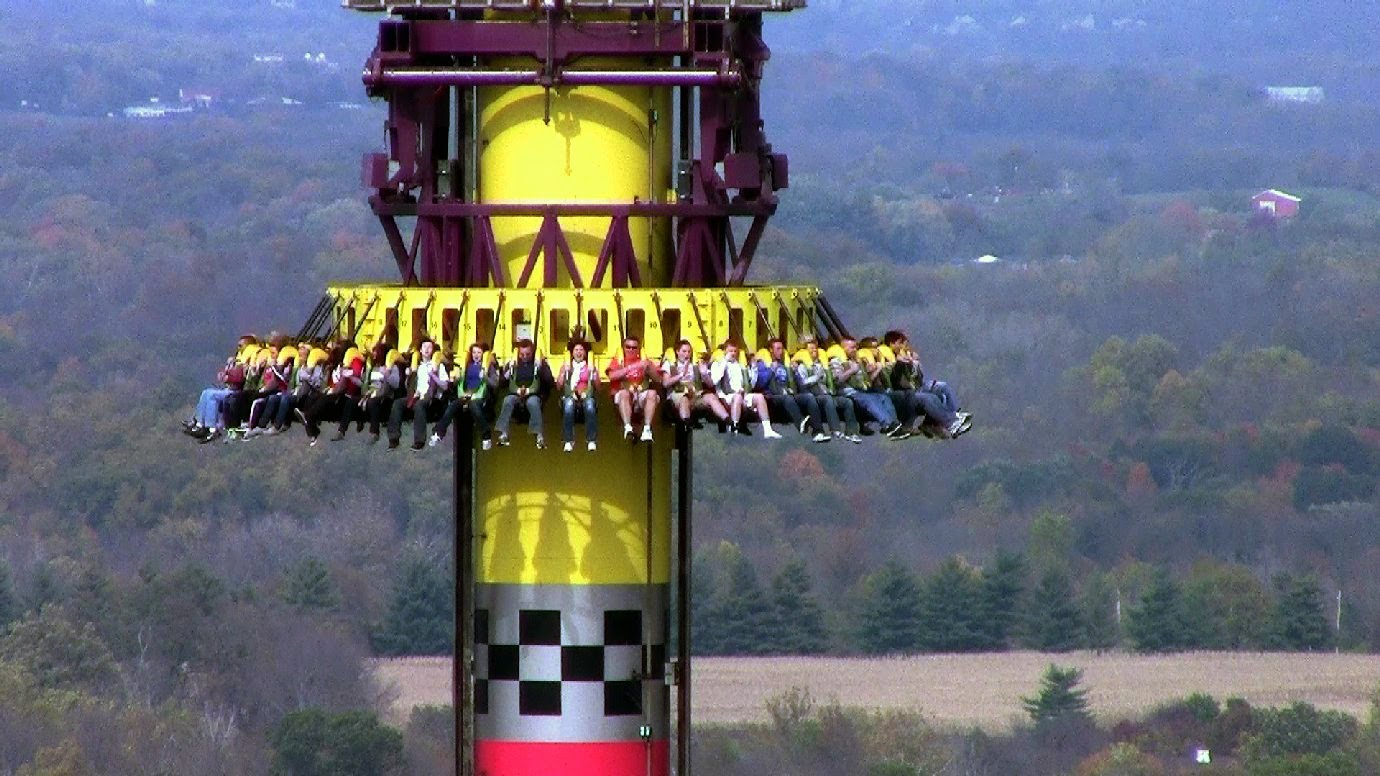
\includegraphics[width=0.4\textwidth]{../images/drop_tower_image.jpg}\end{center}
	\vspace{-20pt}
\end{wrapfigure}

\question \textbf{Drop Tower:} At theme parks, there is a kind of ride known as a \textit{drop tower.} People (safely strapped in harnesses) rise to the top of a large tower, and are then dropped down to experience free fall. The image to the right shows a picture of people on the drop-tower ride at Kings Island.

The graph below shows someone's \textit{velocity as a function of time} as they rise to the top (from 0 to 41 seconds), pause at the top not moving (from 41 to 52 seconds) and then falling (from 52 to 60 seconds). In all, the ride lasts exactly 1 minute.

\noindent\begin{center}
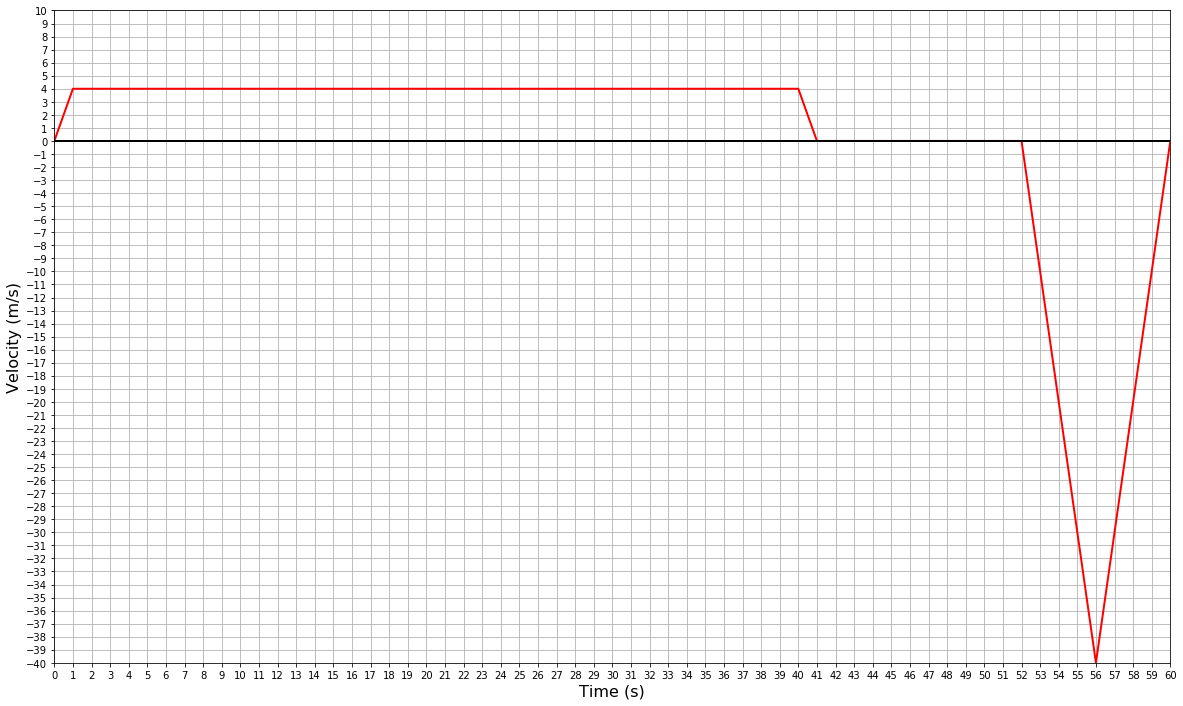
\includegraphics[width=0.9\textwidth]{../images/test1V1_dropTower.png}
\end{center}

\begin{parts}
	\part[2] When is \textit{acceleration zero} during the ride? Provide all time interval(s).
		\vspace{1in}
	\part[2] When do people experience free fall during the ride (i.e. are accelerating solely due to gravity)? Provide all time interval(s).
		\vspace{1in}
	\part[2] How high is the tower?
		\vspace{1in}
\end{parts}
\end{minipage}

\clearpage

\bonusquestion[4] List 4 problems with science.
\fillwithlines{4in}

\clearpage
This page is left blank for calculations.

\clearpage
This page is left blank for calculations.

\clearpage
This page is left blank for calculations.


\end{questions}


\end{document}